\documentclass{beamer}
\usetheme{afm}

\title{Monte Carlo Simulation and Stochastic Processes}
\author{\href{mailto:matteo.sani@unisi.it}{Matteo Sani}}

\begin{document}
\begin{frame}[plain]
	\maketitle
\end{frame}

\begin{frame}[fragile]{\textttdDatetime}}
    \begin{itemize}
      \item We will frequently use \texttt{datetime} module, which is dedicated to date and time in \texttt{python}.
      \item In addition we rely on \texttt{dateutil.relativedelta} to perform operations on dates (dedicated Sections in the notes).
    \end{itemize}
\begin{ipython}
from datetime import date
from dateutil.relativedelta import relativedelta

d = date.today()
print (d)

d1 = date(2023, 12, 25)
print (d1)
print ((d1 - d).days)
print (d1.strftime('%d/%m/%Y'))
print (d1.weekday())
print (d + relativedelta(days=45))
print (d + relativedelta(months=45))
\end{ipython}
\begin{ioutput}
2022-09-27
2023-12-25
454
25/12/2023
0
2022-11-11
2026-06-27
\end{ioutput}
\end{frame}

\begin{frame}[fragile]{Payment Dates Generator}
  \begin{itemize}
    \item Since we will need to create many lists of dates (e.g. contract payment dates) let's develop an utility that does that for us.
    \item The function takes as input
      \begin{itemize}
        \item \emph{starting date} (the first date of the list);
        \item \emph{maturity} a string like \texttt{5y} or \texttt{17m} which represents the length of the list;
        \item \emph{tenor} string like maturity with default value of \texttt{12m}, if the maturity is not a multiple of the tenor the last period will be truncated to the last date.
      \end{itemize}
    \item The function returns a list of dates.
\begin{ipython}
!pip install --index-url https://test.pypi.org/simple finmarkets
\end{ipython}

\begin{ipython}
from datetime import date
from dateutil.relativedelta import relativedelta
from finmarkets import maturity_from_str

def generate_dates(start_date, maturity, tenor="1y"):
  maturity_months = int(round(maturity_from_str(maturity), 0))
  tenor_months = int(round(maturity_from_str(tenor), 0))
  dates = []
  for d in range(0, maturity_months, tenor_months):
    dates.append(start_date + relativedelta(months=d))
  dates.append(start_date + relativedelta(months=maturity_months))
  return dates

print (generate_dates(date.today(), "25m"))
\end{ipython}
\begin{ioutput}
[datetime.date(2023, 8, 28), datetime.date(2024, 8, 28), datetime.date(2025, 8, 28), datetime.date(2025, 9, 28)]
\end{ioutput}
\enf{frame}

\begin{frame}{Object Oriented Programming (OOP)}
  \begin{itemize}
  \item OOP is a programming model where programs are organized around data, or **objects**, rather than functions and logic.
  \item Every object can be thought of as a dataset with unique attributes and behaviour.
  \item Examples:
    \begin{itemize}
    \item a human being that is described by properties like name and birthday;
    \item the \emph{abstract concepts} of a discount curve with dates and discount factor.
    \end{itemize}
  \end{itemize}
\end{frame}

\begin{frame}{Classes}
  \begin{itemize}
    \item Classes are the key ingredient of \emph{Object Oriented Programming}.
    \item They are implemented in many modern programming language like \texttt{python}, \texttt{Java}, \texttt{C++}\ldots
    \item In the OOP framework, classes are meant for
      \begin{itemize}
        \item creating objects (a particular data structure);
        \item providing initial values for its state (member variables or attributes);
        \item implementing their behaviour (member functions or methods).
      \end{itemize}
    \item \textbf{A class allows to bundle data and methods that work on that data within one single object.}
    \item At the very end \emph{classes} are collections of functions that operate on a dataset and \emph{instances} of that class represent individual datasets (or if you prefer a *specialization* of that class).
  \end{itemize}
\end{frame}

%![](https://drive.google.com/uc?id=1jAxUvetAM5HVv4yT_xYaFgCvxj8OEI8J)

\begin{frame}{Discount Curve Class}
  \begin{itemize}
    \item Import the necessary modules;
    \item then the \texttt{class} keyword followed by a name is used to start the actual definition;
    \item define the \emph{constructor} method:
      \begin{itemize}
        \item it is always named as \texttt{__init__};
        \item \textbf{as every other method in a class, takes \texttt{self} as the first argument};
        \item then any number of parameters as desired by the programmer.
      \end{itemize}
    \item \texttt{__init__} allows to specify the initial state of a class by setting its attribute values;
    \item here, talking about a possible driver, we may want to specify its name and birthday.
  \end{itemize}
\end{frame}

\begin{frame}{Discount Curve Class}
  \begin{itemize}
  \item \textbf{Attributes} (characteristic data for a curve):
    \begin{itemize}
      \item list of pillar dates (corresponding to the given discount factors), $t_0,...,t_{n-1}$;
      \item list of discount factors, $D(t_0),...,D(t_{n-1})$.
    \end{itemize}
  \item \textbf{Methods} ("behaviour" of a discount curve):
    \begin{itemize}
    \item one single method returning a discount factor at a given date (if necessary it must interpolate between existing factors);
    \item the method will use a log-linear interpolation.
    \end{itemize}
    \begin{equation*}
      d(t_i)=\log(D(t_i)) = \log(e^{-r(T-t_i)}) = -r(T-t_i) \;\;\textrm{where $i$ is such that}\;t_i \le t \le t_{i+1}$$  
    \end{equation*}
  \end{itemize}

\begin{frame}{Class Definition}
\begin{ipython}
import numpy as np

from datetime import date
from scipy.interpolate import interp1d  

class DiscountCurve:
  def __init__(self, obs_date, pillar_dates, discount_factors):
#      self.obs_date = obs_date
      if obs_date not in pillar_dates:
          pillar_dates = [obs_date] + pillar_dates
          discount_factors = np.insert(np.array(discount_factors), 0, 1)
      pillar_dates = [d.toordinal() for d in pillar_dates]
      self.interpolator = interp1d(pillar_Dates, np.log(discount_factors))
          #self.log_discount_factors = [np.log(discount_factor) for discount_factor in self.discount_factors]
    #self.pillar_days = [(pillar_date - obs_date).days for pillar_date in self.pillar_dates]
\end{ipython}
\begin{itemize}
\item Variables whose name starts with \texttt{self.} have \emph{class scope}, i.e. are available within each class method.
\item Class attributes have to be defined as \texttt{self.variableName = param}
\item The \texttt{self.} prefix is used to create and access every attribute or method from within the class itself.
\end{frame}

\begin{frame}{Class Instantiation}
\begin{itemize}
  \item Now that we have the class definition that represents a \emph{generic} discount curve we can specialized it to some \emph{real} curve.
  \item When \emph{instantiating} a class, \texttt{python} first calls the \texttt{__init__} method and initializes the attributes with the parameter we are passing.
  \item \textbf{To access class attributes and methods the dot (.) operator has to be used.}
\begin{ipython}
from finmarkets import generate_dates

pillars = generate_dates(date.today(), "5y")
dfs = [1, 0.98, 0.97, 0.96, 0.95, 0.94]      
dc = DiscountCurve(date.today, pillars, dfs)
print (dc.interpolator.x) # pillars
print (dc.interpolator.y) # log dfs
\end{ipython}
\begin{ioutput}
<class '__main__.Driver'>
Matteo
1974-10-20
\end{iotuput}
\end{itemize}
\end{frame}

\begin{frame}{Class Methods}
  \begin{itemize}
  \item We haven't yet defined any \emph{curve behaviour}, so let's add a methods computing the discount factor at a given datep.
    \begin{iptyhon}
import numpy as np

from datetime import date
from scipy.interpolate import interp1d  

class DiscountCurve:
  def __init__(self, obs_date, pillar_dates, discount_factors):
      if obs_date not in pillar_dates:
          pillar_dates = [obs_date] + pillar_dates
          discount_factors = np.insert(np.array(discount_factors), 0, 1)
      pillar_dates = [d.toordinal() for d in pillar_dates]
      self.interpolator = interp1d(pillar_Dates, np.log(discount_factors))

  def df(self, d):
      d_to = d.toordinal()   
      if d_to < self.interpolator.x[0] or d_tp > self.interpolator.y[-1]:
            print (f"Cannot extrapolate discount factors (date: {d}).")
            return None
        return np.exp(self.interpolator(d_to)
\end{ipython}

%* **As the problem complexity increases more lists and helper functions are needed with the latter approach and soon the program becomes difficult to be maintained.**





from datetime import date
from finmarkets import generate_dates
from scipy.interpolate import interp1d 

pillars = generate_dates(date.today(), "5y")
dfs = [1, 0.98, 0.97, 0.96, 0.95, 0.94]

def df(d, pillars, dfs):
  interp = interp1d(pillars, dfs)
  return interp(d)

print (df(date(2024, 3, 15), pillars, dfs))
---------------------------------------------------------------------------
ValueError                                Traceback (most recent call last)
<ipython-input-6-9b45c0e87d11> in <cell line: 12>()
     10   return interpolator(d)
     11 
---> 12 print (df(date(2024, 3, 15), pillars, dfs))

3 frames
/usr/local/lib/python3.10/dist-packages/scipy/_lib/_util.py in _asarray_validated(a, check_finite, sparse_ok, objects_ok, mask_ok, as_inexact)
    253     if not objects_ok:
    254         if a.dtype is np.dtype('O'):
--> 255             raise ValueError('object arrays are not supported')
    256     if as_inexact:
    257         if not np.issubdtype(a.dtype, np.inexact):

ValueError: object arrays are not supported

pillars = generate_dates(date.today(), "5y")
dfs = [1, 0.98, 0.97, 0.96, 0.95, 0.94]

def df(d, pillars, dfs):
  d = d.toordinal()
  pillars = [d.toordinal() for d in pillars]
  interp = interp1d(pillars, dfs)
  return interp(d)

print (df(date(2024, 3, 15), pillars, dfs))
  
0.9890710382513661  









    
\begin{frame}{Random Variables}
    \begin{columns}
    \column{0.3\textwidth}
    When the range of possible values for $X$ is infinite it is called a \emph{continuous}; contrary it is \emph{discrete}.
    \column{0.7\textwidth}
    \begin{figure}[h]
    \begin{center}
    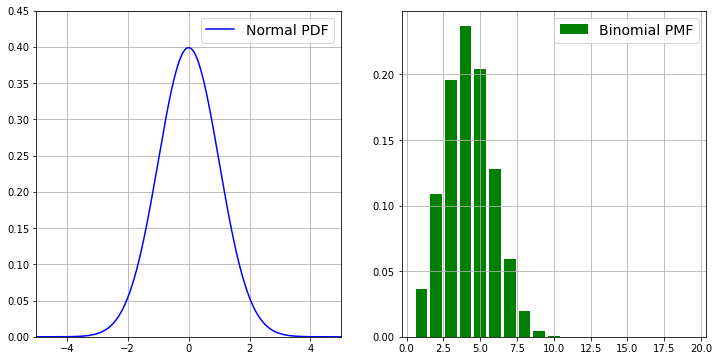
\includegraphics[width=1.0\linewidth]{rv_pdf}
    \end{center}
    \end{figure}    
    \end{columns}
\end{frame}

\begin{frame}{CDF and Quantiles}
	\begin{itemize}
    \item The cumulative distribution function (CDF) $F$ of a random variable $X$ (with PDF $f(x)$, evaluated at $x$, is the probability that $X$ will take a value less than or equal to $x$
    \begin{equation*}
        \begin{gathered}
            F_X(x) = Pr(X\leq x) = \int_{-\infty}^{x} f(x)dx\\
            Pr(a \leq X\leq b) = \int_{-\infty}^{b} f(x)dx - \int_{-\infty}^{a} f(x)dx = \int_{a}^{b} f(x)dx
        \end{gathered}
    \end{equation*}
    
    \item The quantile function $Q$, associated with a probability distribution of a random variable, and evaluated in $p$ specifies the value $x$ of the random variable such that the probability $p$ of the variable being less than or equal to that value equals the given probability. 
    \begin{itemize}
        \item It is also called the percent-point function (PPF) or inverse cumulative distribution.
    \end{itemize}
    \begin{equation*}    
        Q_X(p) = F_X^{-1}(X \leq x_p)\;\;\textrm{where}\; F_X(x_p) = p
    \end{equation*}
    
    \item The quantile function does the "inverse" of the cumulative distribution function.
	\end{itemize}
\end{frame}

\begin{frame}{CDF and Quantiles}
    \begin{figure}[h]
    \begin{center}
    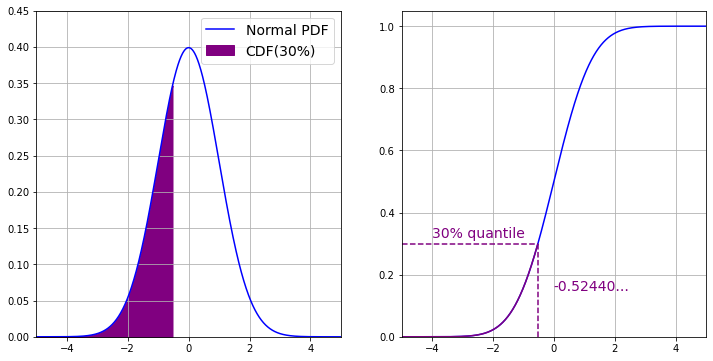
\includegraphics[width=0.7\linewidth]{cdf_quantiles}
    \end{center}
    \end{figure}    
\end{frame}

\begin{frame}[fragile]{PDFs in \texttt{python}}
    Many distributions are implemented in \texttt{scipy} package,
\begin{ipython}
from scipy.stats import norm, binom
     
norm.pdf(0)   				# evaluate the PDF in 0
binom(12, 0.35).pmf(2)		# evaluate the PDF in 0
norm.cdf(0)					# compute the CDF up to 0
norm.ppf(0.3)               # return the 0.3 quantile
norm.rvs(size=100)          # sample 100 times from normal distribution
\end{ipython}
\end{frame}

\begin{frame}{Monte Carlo Simulation}
    \begin{itemize}
    \item Monte Carlo (MC) methods are a broad class of computational algorithms that rely on repeated random sampling to obtain numerical results
    \begin{itemize}
        \item use randomness to solve problems that might be deterministic in principle;
        \item used when a closed-form solution for a property being studied cannot be developed (i.e. the probability of varying outcomes cannot be determined because of random variable interference). 
     \end{itemize}
    \item In Monte Carlo each random variable of a model is "replaced" with their PDF; the outcome of the model is then computed many times with different samples of the random variables. 
    \item In finance MC has a vast array of potential applications
    \begin{itemize}
        \item to estimate the likelihood that an asset price will move in a certain way;
        \item to assess the risk that an entity will default;
        \item to analyze derivatives such as options.
     \end{itemize}
    \item MC simulations have also countless applications in gaming, meteorology, astronomy, physics...
    \end{itemize}
\end{frame}

\begin{frame}{Algorithm Description}
    \begin{enumerate}
    \item Identify the random variables of the problem and define the domain $\Omega$ of possible inputs (probability distributions for each random variable);
    \item generate random samples from the domain $\Omega$;
    \item compute the model output based on the randomly generated inputs;
    \item repeat the experiment $N$ times and "aggregate" the results.
    \end{enumerate}
    \begin{block}{Example}
    Simulate results of rolling a die. The random variable describe the die outcome, hence $\Omega = {1,2,3,4,5,6}$ with uniform PDF (fair die).
    The simulation consists of sampling uniform distributed integers between 1 and 6.
    \end{block}
\end{frame}

\begin{frame}{Pseudo-Random Numbers}
    \begin{itemize}
    \item  Depending upon the number of uncertainties and their PDFs, a Monte Carlo simulation could involve thousands or even tens of thousands of recalculations.
    \item For each simulation large amounts of random numbers sampled from many different probability distributions are computed, hence the widespread of this method spurred the development of pseudo-random number generators. 
    \item Every programming language has libraries that allows to produce huge series of random numbers:
    \begin{itemize}
        \item those numbers are generated by algorithms that take as input a *seed* which determines univokely the series; 
        \item setting the same seed produce the same set of numbers every time (which is great for debugging purpouses).
    \end{itemize}
    \end{itemize}
\end{frame}

\begin{frame}[fragile]{Pseudo-Random Numbers}  
\begin{ipython}
import random 

random.seed(1)
print(random.random())       # 0.13436424411240122
print(random.random())       # 0.8474337369372327

random.seed(2)
print(random.random())       # 0.9560342718892494
print(random.random())       # 0.9478274870593494

random.seed(1)
print(random.random())       # 0.13436424411240122
print(random.random())       # 0.8474337369372327

print (random.randint(1, 6)) # 1
a = ['a', 'b', 'c', 'd']
print (random.sample(a, 2))  # ['c', 'a']
\end{ipython}
\end{frame}

\begin{frame}[fragile]{Estimate Distributions}
The \texttt{random} module has also some limited capabilities for sampling from a distribution, anyway 
better to use \texttt{scipy}.

\begin{columns}
\column{0.5\linewidth}
\begin{ipython}
import numpy as np
from random import randint
from scipy.stats import uniform, norm

# uniform distribution
numbers = []
for _ in range(10000):
    numbers.append(randint(0, 5))

# normal distribution
norm.rsv(size=100000)   
\end{ipython}
\column{0.5\linewidth}    
\begin{figure}[h]
    \begin{center}
    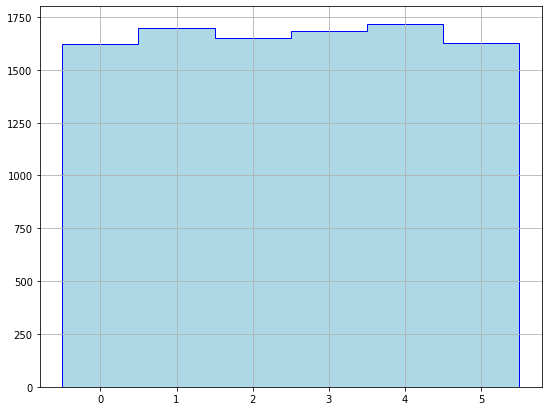
\includegraphics[width=0.55\linewidth]{uniform_distro}\\
    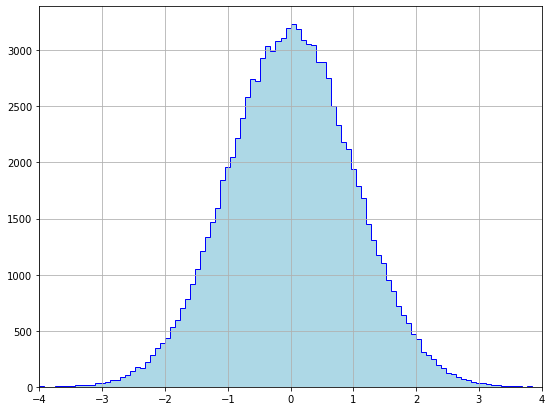
\includegraphics[width=0.55\linewidth]{gauss_distro}
    \end{center}
\end{figure}    
\end{columns}
\end{frame}

\begin{frame}{Monte Carlo Simulation}
\begin{block}{Example}
Measure probability to get two kings drawing randomly two cards from a deck.
\begin{equation*}
P_{\textrm{two kings}} = \frac{4}{40} \cdot \frac{3}{39} = \frac{1}{130} \approx 0.007692
\end{equation*}
This analytical results can be reproduced with a Monte Carlo simulation by taking a frequentist approach
\begin{equation*}
\textrm{probability of event} = \cfrac{\textrm{n. successes}}{\textrm{n. experiments}}
\end{equation*}
\end{block}
\end{frame}

\begin{frame}{Monte Carlo Simulation Example}
\begin{itemize}
    \item In the example we ran 10000 simulations and obtained a probability of 0.7\% (it means on average we get 2 kings once every 700 draws).
    \item \emph{The precision of the result depends on the number of "successes".}
    \item Imagine to run only 100 experiments, it is highly probable that I get no successes at all, should I conclude there is a 0 probability to get 2 kings ?
    \item The lower is the probability for a successful experiment the higher has to be the number of simulations, if the probability is small, we need to try many times.
    \item Monte Carlo Simulation is not always the best approach to follow !
\end{itemize}
\end{frame}

\begin{frame}{Accuracy of Monte Carlo Simulation}
Imagine you don't know the probability of getting two consecutive K from a deck: what can be concluded from the result of a single MC experiment ?
\begin{block}{Central Limit Theorem}    
If $Y_1, Y_2,\dots, Y_n$ are $n$ random samples from a distribution $Y$ with true mean $\mu$ and variance $\sigma^{2}$, then when $n$ is sufficiently large, 
\begin{equation*}
\mu_n = \cfrac{1}{n}\sum_i^n Y_i \approx \mathcal{N}(\mu, \sigma^2/n)
\end{equation*}
has approximately a normal distribution $\mathcal{N}(\mu, \sigma^2/n)$. 

This means that if ones repeats a MC experiment (changing the seed of the random number generator) she should obtain results normally distributed around the \emph{true} value $\mu$.
\end{block}
\end{frame}

\begin{frame}{Confidence Interval}
\begin{itemize}
\item Since
\begin{equation*}
\mu_n \approx \mathcal{N}(\mu, \sigma^2/n)\implies \mu_n - \mu \approx \mathcal{N}(0, \sigma^2/n)
\end{equation*}
we can define an interval such that there is a given probability to find $\mu$ in there.
\begin{columns}
\column{0.5\linewidth}
\begin{equation*}
P\left(\mu_n - 1.96\frac{\sigma}{\sqrt{n}}\le \mu \le \mu_n + 1.96\frac{\sigma}{\sqrt{n}}\right) = 0.95
\end{equation*}
\column{0.5\linewidth}
\begin{figure}[h]
    \begin{center}
    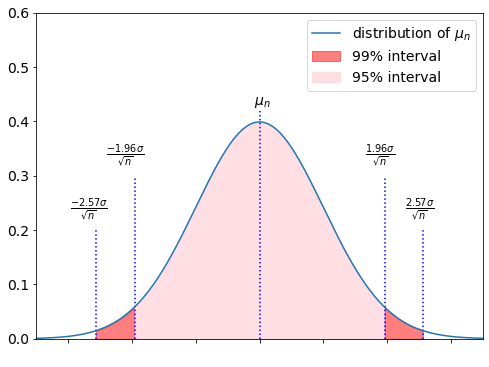
\includegraphics[width=0.8\linewidth]{confidence_interval_pink}
    \end{center}
\end{figure}    
\end{columns}
\item This is the \emph{95\% confidence interval} since pink area is 95\% of the area under the Gaussian.
\item Repeating many times a simulation, the fraction of confidence intervals containing the true $\mu$ would tend toward 95\%.
\end{itemize}
\end{frame}

\begin{frame}[fragile]{Confidence Interval}
The most common intervals are 99\% and 95\% confidence levels and are respectively defined as $\pm \cfrac{2.57\sigma}{\sqrt{n}}$ and $\pm \cfrac{1.96\sigma}{\sqrt{n}}$. 
\begin{ipython}
import numpy as np

cl = 1.96*np.std(r)/np.sqrt(experiments)
print (f"{np.mean(r):.6f} +- {cl:.6f} @ 95% confidence level")
# 0.007689 +- 0.000054 @ 95% confidence level
\end{ipython}
\end{frame}

\begin{frame}[fragile]{Standard Deviation of the Mean}
\begin{itemize}
\item To get further information about the precision of our estimate $\mu_n$, or about the accuracy of the Monte Carlo simulation in general, we can use the standard deviation of the sampled mean. 
\item Assuming statistical independence of the values in the sample, the standard deviation of the mean is 
\begin{equation*}
\sigma _{\text{mean}}={\frac {1}{\sqrt {n}}}\sigma
\end{equation*}
where $n$ is the number of observations in the sample used to estimate the mean. 

\begin{ipython}
print (f"{np.mean(r):.6f} +- {np.std(r)/np.sqrt(experiments):.6f}")
# 0.007689 +- 0.000028
\end{ipython}
\item To get one more digit of accuracy (i.e. an error one tenth as large) requires a $\times100$ simulations.
\item To get three more digits of accuracy requires one million times as much computation: \emph{running 10000 above experiments ($\times10$ more) gives an error 3 times smaller (from 2.8e-5 to about 9e-6)}.
\end{itemize}
\end{frame}

\begin{frame}{Stochastic Processes}
\begin{itemize}
\item \emph{Deterministic process}: all data necessary to predict the system development with 100\% certainty is available.
\item \emph{Stochastic or random process}: exhibits behaviors that cannot be described by a deterministic model, is a \emph{noisy} process where uncertainty needs to be modeled
   \begin{itemize}
    \item it is a collection of random variables indexed by some set (usually time);
    \item each random variable of the stochastic process is uniquely associated with an element in the set. 
    \end{itemize}
\begin{figure}[h]
    \begin{center}
    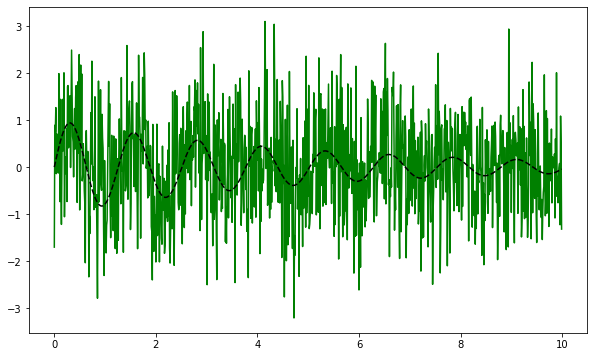
\includegraphics[width=0.5\linewidth]{stochastic_process}
    \end{center}
\end{figure}        
\end{itemize}
\end{frame}

\begin{frame}{Stochastic Processes}
\begin{itemize}
\item Stochastic processes are described by \emph{stochastic differential equation (SDE)}:
\begin{equation*}
dX(t) = \mu(t,X(t)) dt + \sigma(t,X(t)) dW(t) = \underbrace{\mu(t,X(t))dt}_{\textrm{deterministic}} + \underbrace{\sigma(t,X(t)) \mathcal{N}(0,1)\sqrt{dt}}_{\textrm{stochastic}}
\end{equation*}
\item The mean of $dW$ is zero and its variance is $dt$
   \begin{itemize}
    \item the standard deviation grows with the square root of time: $W(t) - \mathcal{N}( 0, t )$ because each $dW$ is distributed like independent standard Gaussian.
    \end{itemize}
\end{itemize}
\begin{figure}[h]
    \begin{center}
    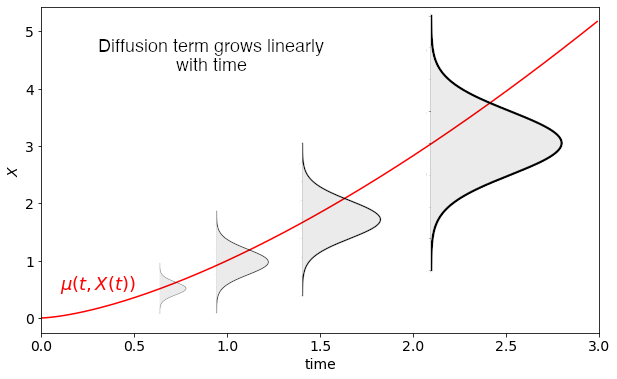
\includegraphics[width=0.50\linewidth]{brownian_process}
    \end{center}
\end{figure}        
\end{frame}

\begin{frame}{Geometric Brownian Motion}
\begin{itemize}
\item Stock prices changes as a result of the random fluctuations given by the trades. The relative change in its price in a period $dt$ can be decomposed into two parts:
\begin{itemize}
    \item \emph{deterministic}, the expected return from the stock hold during the time period $dt$ ($\mu S_tdt$);
    \item \emph{stochastic} which reflects the random changes of the market (e.g. as a response to external effects such as unexpected news). A reasonable assumption is to take this contribution proportional to the stock ($\sigma S_t dW_t$).
\end{itemize}
\begin{equation*}
dS_t = \mu S_tdt + \sigma S_tdW_t;\quad\frac{dS_t}{S_t} = d\textrm{log}(S_t) = \mu dt + \sigma dW_t 
\end{equation*}
\item The solution of this SDE can be derived by applying the It$\hat{o}$'s formula (full derivation in the notes).
\begin{equation*}
S_t = S_{t-1}e^{\big(\mu - \frac{1}{2}\sigma^2\big)dt + \sigma Z\sqrt{dt}}
\end{equation*}
\end{itemize}
\end{frame}

\begin{frame}{Geometric Brownian Motion}
\begin{itemize}
\item The change in $\textrm{log} S_t$ has a constant \emph{drift} $\mu - \frac{1}{2}\sigma^2$ and a constant variance rate $\sigma^2$ (remember that $Z=\mathcal{N}(0,1)$) therefore $\textrm{log} S_t$ at some time $T$ is normally distributed with:
\begin{equation*}
\textrm{log}\left(\cfrac{S_t}{S_{t-1}}\right) = \left(\mu - \frac{1}{2}\sigma^2\right)dt + \sigma Z\sqrt{dt} \approx\mathcal{N}\left[\left(\mu-\frac{\sigma^2}{2}\right)T, \sigma^2 T\right]
\end{equation*}
\end{itemize}
\begin{block}{}
A variable whose logarithm is normally distributed is said to be \emph{log-normal}, lognormality is important because ensures a stock price will never be negative.
Looking at the initial $dS$ equation we had that:
\begin{equation*}
dS_t = \mu S_tdt + \sigma S_tdB_t
\end{equation*}
which shows that the closer is $S_t$ to 0 the smaller is the $dS$ variation (so it will never go below 0).
\end{block}
%\begin{figure}[h]
%    \begin{center}
%    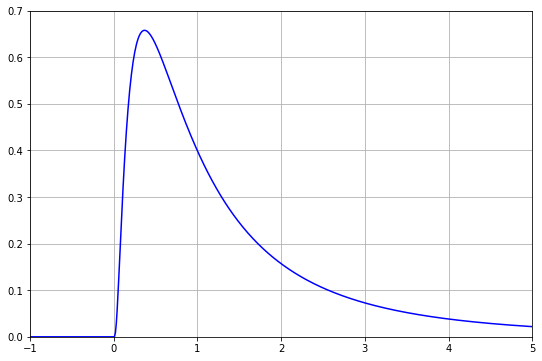
\includegraphics[width=0.7\linewidth]{lognormal}
%    \end{center}
%\end{figure}        
\end{frame}

\begin{frame}{Simulating SDE}
\begin{itemize}
\item  Consider the generic SDE
\begin{equation*}
dX(t) = \mu(t,X(t))dt + \sigma(t,X(t))dW(t)
\end{equation*}
the simulation of $X(t)$ is done as follows.
\item Starting from the value of $X(t_i)$ compute $X(t_{i+1})$ using the given SDE by setting $\Delta t = t_{i+1} - t_{i}$, and sampling from a standard normal $\mathcal{N}(0,1)$
\begin{equation*}
X(t_{i+1}) = X(t_i) + \mu(t_i,X(t_i))\Delta t + \sigma(t_i,X(t_i))\sqrt{\Delta t}\mathcal{N}(0,1)
\end{equation*}
\end{itemize}
\end{frame}

\begin{frame}{Remark on Stochastic Processes}
\begin{itemize}
\item Whenever we want to estimate a quantity involving stochastic processes we have to compute an expectation $\mathbb{E}[f(X)]$.
\item This means that we have to average the value of $f(X)$ among all the possible realizations of $X$ taking into account the probability associated to each path.
\item Monte Carlo simulation is a way of estimate an expectation: 
\begin{enumerate}
\item simulate as many $X$ realization as possible;
\item for each simulation compute $f(X)$;
\item average the results to estimate $\mathbb{E}[f(X)]$.
\end{enumerate}
\end{itemize}
\end{frame}

\end{document}
